\documentclass[aps,prl,reprint,amsmath,amssymb,nature]{revtex4-1}

% define variable that compiles the main text (as opposed to SI text)
\newcommand*{\MAINTEXT}{}

\usepackage{epsfig,color,graphicx}

\begin{document}
\newcommand{\Ang}{\ensuremath{\mathring{\text{A}}}}
\newcommand{\red}{\color{red}}
\newcommand{\blue}{\color{blue}}
\newcommand{\old}{\color{black}}

\bibliographystyle{naturemag}

%\ifdefined\MAINTEXT
%\else
%	\clearpage
%	%\widetext
%	\setcounter{figure}{0}
%	\setcounter{page}{1}
%	\renewcommand{\thefigure}{S\arabic{figure}}
%\fi

\title{
\ifdefined\MAINTEXT
\else
Supplementary Information: \\
\fi
Machine learns the physics of intermolecular interactions
}

\author{Volodymyr Sakun}
\affiliation{Department of Civil Engineering, McGill University, 817 Sherbrooke St. West, Montreal, QC H3A 0C3, Canada}
\author{Rustam Z. Khaliullin}
\email{rustam.khaliullin@mcgill.ca}
\affiliation{Department of Chemistry, McGill University, 801 Sherbrooke St. West, Montreal, QC H3A 0B8, Canada}

\date{\today}

\ifdefined\MAINTEXT

\begin{abstract}
\red Abstract is to be written once we finish the main text. Many journals have a 150-word limit on abstract. 
IMO, best abstracts contain no more than 5 sentences. \old
\end{abstract}

\maketitle


\section{Introduction}

Machine learning shows enormous promise for modeling of materials and molecules~\cite{ceriotti-science}. 
One of the many rapidly growing area of its application is the development of interatomic potentials---functions that describe the dependence of the interaction energy between atoms on their positions. 
In the last decade, several approaches based on artificial neural networks (ANNs) and Gaussian process regression (GPR) have been 
developed to approximate interatomic potentials using accurate quantum mechanical data as training data. 
The main advantage of carefully calibrated machine-learned potentials (MLPs) is that they combine the high accuracy of quantum mechanical description of interaction between atoms with the computational efficiency of simple human-derived analytical potentials. 
%This rare combination of accuracy and cost has enabled high-quality MLP-based simulations of complex materials on unprecedented time and length scales~\cite{Khaliullin2010,Khaliullin2011,RZK0}. 
Being the key component for atomistic modeling, MLPs with their rare combination of accuracy and cost have enabled simulations of complex materials on unprecedented time and length scales~\cite{Khaliullin2010,Khaliullin2011,RZK0}. 

%RZK0: Describe the main principles of local descriptors and similarity measure, so that the introduction below is clear.

The high accuracy of MLPs is the result of a very flexible form of the model energy function, parametric or nonparametric. 
This flexibility allows the learning algorithm to adjust the model in order to reproduce the known energies at the training points and then \textit{interpolate} between the points thus predicting the energies for new structures. 
Unfortunately, the accuracy of the existing MLPs comes with poor transferability. Machine-learning algorithms are unable to \textit{extrapolate} the energy function to the atomistic configurations that do not resemble those in the training set.
The transferability problem arises not only for configuration that lie \emph{outside}---according to some distance measure---the training set but also may appear for configurations \emph{inbetween} training points. 
A typical example of the former case is an MLP trained to reproduce the energies for a material in a certain pressure interval that fails dramatically for any pressure outside this range. 
The latter situation occurs when the training set is too sparse for accurate interpolation. For example, an MLP trained on configurations collected from liquid phases might not be able to predict energies of its crystal phases even though the local structures in liquid resembles those in solid state. 
In order to cope with the sparsity problem, training sets must include accurate quantum mechanical energies for a large number of representative atomistic configurations.%, making the training process computationally unfeasible.

While the accuracy-transferability problem plagues many human-derived energy models it is particularly severe in the case of MLPs. 
For MLPs, the transferability issues summarized above stem from the complete neglect of the physics of interaction between atoms. 
For example, ANNs rely on unphysical sigmoid functions, whereas GPR can be viewed as a nonparametric energy representation in a set of unphysical Gaussian functions. 
Thus MLPs are designed as very flexible universal approximators that just \emph{mimic} the functional shape of complex interatomic potentials. 

The severity of the transferability problem has inspired numerous attempts to put the physical components back into MLPs. 
The resulting hybrid approach uses fixed human-derived analytical potentials, in which parameters are now obtained with machine-learning algorithms. 
While such a scheme can extend the transferability and range of applications of a potential, its fixed analytical form reduces the accuracy of predictions.

In this work, we propose a different approach to learning interatomic potentials that aims at improving their transferability without compromising the flexibility and accuracy. 
%The key idea of the methodology presented here is to let the algorithm select, out of a multitude of physically appropriate functions, only those few that reproduce the training data best. 
The key idea of the methodology described here is to represent the energy model by a multitude of physically appropriate trial functions and then let the learning algorithm select only those few that reproduce the training data best. 
A large number of the trial energy functions ensures the accuracy of the model. 
The physics built into the model and the tight control of overfitting improve its transferability. 
Furthermore, the Occam's razor principle applied to the learning process produces simple analytical energy expressions that resemble those describing fundamental physical laws. 
The obtained physically motivated analytical equations can properly describe interactions between atoms outside the training set. 
To demonstrate a feasibility of the outlined approach, we considered only intermolecular interactions, for which physically relevant energy models can be constructed with linear functions.

\section{Methodology}

%\red Short description of the general methodology with only basic equations and motivation behind them. All examples related to a specific model (e.g. water) will be presented in Results and Discussion. Description of the code (not be confused with algorithm) should be moved to the Supplementary Information. All results should be presented in Results and Discussion, unless they are necessary to understand our methodology. \old

This expression also satisfies another important physical constraints: it makes energy invariant to translations and rotations of the entire molecular system. 

For any system, the potential energy as a function of interatomic distances satisfies two constraints: it approaches zero when all atoms are infinitely far from each other and it becomes infinite as the distance between any two atoms approaches zero.
%
\begin{eqnarray}
\lim_{\forall R_i \rightarrow \infty} E (\mathbf{R}) = 0 \\
\lim_{R_i \rightarrow 0} E (\mathbf{R}) = \infty
\end{eqnarray}

Define: Features

We chose powers of inverse distances (POIDs) as a set of [features] because their sum can easily satisfy these two very general physical constraints:
\begin{eqnarray}
E (&R_1&, R_2, \ldots, R_N) = \sum_{k=1}^{M_1} \sum_{p=1}^{N} \frac{c_{pk}}{R_p^k} + \sum_{k,m=1}^{M_2} \sum_{p>q}^{N} \frac{c_{pkqm}}{R_p^k R_q^m} + \nonumber \\
&+& \ldots +\sum_{k,m,n=1}^{M_G} \sum_{p>q>r}^{N} \frac{c_{pkqm\ldots rn}}{R_p^k R_q^m \ldots R_r^n} \equiv \mathbf{f}\cdot \mathbf{c}
\end{eqnarray}
%
where $N = \frac{1}{2}A(A-1)$ is the number of distances $R$ between $A$ atoms, M$_{g}$ is the maximum power for a term containing the product of $g$ distances, $G$ is the maximum ZZZ, $\mathbf{c}$ is the vector of tunable coefficients, $\mathbf{f}$ is the vector of features. 
\red To make training flexible/ distances are classified as intermolecular and intramolecular. \old 
In order to account for the equivalence of atoms of the same element and to make sure that the energy is invariant to permutation of atoms in the input, the fitting coefficients for the physically equivalent features are restricted to be equal. 
Taking this symmetry into account allows to decrease the number of independent features in the model and training time substantially. 
For example, the energy of two water molecules depends on 15 distances, only five of which are unique: oxygen-oxygen, intermolecular oxygen-hydrogen, intramolecular oxygen-hydrogen, intermolecular oxygen-hydrogen, intramolecular hydrogen-hydrogen.

Despite satisfying a variety of constraints, expression (3) remains very general. 
The multipole expansion of intermolecular energies implies that POIDs can adequately represent a wide variety of intermolecular potentials. 
The flexibility of the model \red is very high\old as it includes many-body beyond simple pairwise interactions through products 
of POIDs.

\textbf{Systems and training set.} 

%Lennard-Jones model.

Two water molecules TIP3P.

Two water molecules, MP2.

Two-molecule and three-molecule water models, with geometries obtained 
from AIMD.

First of all, the data must contain enough records to cover all possible arrangements that exist in real life. 
In other words, data must contain enough configurations with varying potential from highest in absolute value to zero. 
Another requirement is that data must be sparse and should have equal records for each representative bin, which is in our 
case average distance between centers of masses. 
So, first part of the algorithm takes required amount of records for each interval and that separates training set and test set. 
Only training set is being using for fitting procedure and only test set is being using for predicting and evaluating the accuracy of the fit and visualizing results. 
In order to analyze the efficiency of predicting algorithm, the number of observations can be reduced to required quantity. 
Some algorithms require data standardization, so before doing anything we have to perform feature scaling for training set in order to have zero mean and unit variance for each feature.

[Related to Models] For three water molecules where we have 9 atoms the total number of 
distances = 9$^{2}$/2 - 9/2 = 36. Using same set of powers (M$_{1
}$=15 and M$_{2}$=7) without feature reduction we would have 
540+17640=18180 features. However, reducing the number of features using 
the describe above technique and discarding all intramolecular distances 
the reduced number of features decreases to only 45+630=675 which is 
much more convenient and manageable for fitting.

[Related to Models] However, calculation of variance influence factors showed that there 
exists very strong multicollinearity between features which indicates 
that products must be included in the model. Similarly, to single 
distances model, if M$_{1}$=0 and M$_{2}$=1, set contains 22 
features and new model has in overall 22+5=27 features. Another 
assumption that has been made that our function depends only on 
intermolecular distances. After performing several fitting procedures 
this assumption has been confirmed by results since fitting algorithm 
discards them almost in all cases. This fact allowed us to reduce the 
number of features even more. To get reasonable fit, the number of 
powers must be increased which will increase the number of features. For 
the model with M$_{1}$=15 and M$_{2}$=7 the number of features 
is 45+245=290 which is more than acceptable for fitting. Without 
performing feature reduction, we would have in total 225+2940=3165 
features (this number of features is the same order of magnitude as that 
of ANNs-based MLPs). In case of two water molecules reasonable fit could 
be obtained using only single distances. However, if we have three water 
molecules, the full model should be used since the simplified one cannot 
give accurate fit. 


\textbf{Training procedure.} In this model, POIDs and their products serve as \textit{features}. 
To find a minimalistic and physically relevant representation of the interatomic potential designed an algorithm that finds a set of the best features while simultaneously tuning their flexible parameters (i.e. linear coefficients in our case) to produce the best fit. 
The training procedure includes two stages: feature selection and fine-tuning. 
\red The second part is the improvement of the subset performed using correlation analysis (CA) and searching for alternate features. \old

$[$OLS$]$. Main equation. Why is OLS bad algorithm for fitting?

We explored the applicability of two methods to perform feature 
selection: elastic net regularization (EN) and genetic algorithm (GA). 
While both algorithms produce almost identical results the advantage of 
$[$the?$]$ genetic algorithm is that it can be easily generalized to 
features with nonlinear fitting coefficients (e.g. exponentially 
decaying functions can be included in the feature list later).

\textit{Elastic net}. Basic idea and main equation

As it was mentioned if there is a group of highly correlated variables, 
then the LASSO selects just one variable from a group and drop the 
others. This is not convenient because in our case LASSO can drop 
important features while keeping less important one. EN can overcome 
this problem since it contains two penalties: linear and quadratic. By 
adjusting the two regularization factors, it is possible to force EN to 
keep dependent features in the model. Later the unnecessary features 
will be removed by another algorithm. Therefore, EN allows to reduce the 
number of features from thousands to hundreds or even less. Next step is 
to reduce the number of features decreased by EN to desired value. It 
can be done by the backwards elimination algorithm (BE), which removes 
the feature Basically, BE removes the worst (less significant feature), 
one at a time, based on criterion provided by fitness function \textit{
F} until the desired number of features is reached:

\textit{F = }

 Since after the reduction of number of features by EN the number of 
observations is much greater than number of variables, so we can use 
ordinary least squares (OLS) as a fitness function and the criterion 
would be minimum squared error (MSE). BE can be used for linear and 
nonlinear features; the only difference is different fitness functions.

\textit{Genetic algorithm.}\textbf{ }Very general description of GA. 
Population of chromosomes improved by iterative mutations and 
corssovers.

We used classic genetic algorithm to select best subset of features from the initial set. Since the number of desired selected features is relatively small and for our model does not exceeds 20 features OLS can be used as a fitness function. The goal of GA is to find the best possible combination of features provided by large feature set. GA itself is been used as a search algorithm; at the beginning it converges relatively fast but very slow at the end. The ideal fitness value is equal to 0. After some iterations (its number depends on many parameters and on dataset as well) GA stops improving its best child, therefore it terminates and gives its best result to A* search. GA contains many parameters that can be varied in order to achieve better performance and faster convergence.\\ 
GA parameters:\\
'GA population size': 100,\\
'GA chromosome size': 15,\\
'GA stop time': 600,\\
'GA max generations': 200,\\
'GA mutation probability': 0.3,\\
'GA mutation interval': [1, 4],\\
'GA elite fraction': 0.5,\\
'GA mutation crossover fraction': 0.5,\\
'GA crossover fraction interval': [0.6, 0.4],\\
'GA use correlation for mutation': False,\\
'GA min correlation for mutation': 0.8,\\
'Random' or 'Best' - rank genes in each chromosome and take most important for crossover.\\
'GA crossover method': 'Random',\\
'Random' or 'Correlated' - pool with candidates for possible replacement created through correlation matrix rule.\\
'GA mutation method': 'Random'\\
            
Stopping criteria are elapsed time, number of iterations and tolerance. 

The main difference from classic GA is that mutation function replaces randomly selected feature with alternate feature from correlation list. 

\textit{Using Pearson correlation coefficients.} In general, our algorithm is designed in such a way that it can deal with strong multicollinearity between features. Since our goal is to reduce the number of POIDs in the fitting function, most common methods of dealing with linear dependent features such as principal component analysis are not applicable. We designed a procedure for eliminating/adding/replacing collinear features with two goals: compact and accurate. To find out how a linear correlation between all our features we calculated the correlation matrix (i.e. matrix of Pearson correlation coefficients). Then we create a list of dependent features for each variable using threshold MinCorrelation = some number between 0 and 1 for cut off. If correlation between two features is greater than MinCorrelation they are considered to be linearly dependent. Suppose we have only 5 features and our correlation matrix looks like in \ref{Correlation_matrix}. If we set MinCorrelation = 0.8 than Variable X1 will have a list of dependent variables $[$X2, X3$]$, X2 will have $[$X1, X3$]$, X3=$>$ $[$X1, X2$]$, X4 and will have empty lists which means X4 is linearly independent within chosen tolerance. The closer MinCorrelation to zero - the greater list of dependent variables, therefore the slower the computation but the more accurate will be the final result. This approach can be useful in two cases: mutation method for GA can be chosen as 'Correlated', so mutating gene will be replaced by another one from the list; A* search uses this list in trials to create successors.

\textit{A* (depth first search tree) algorithm}. Its goal is keeping the number of predictors find better subset of features that have better fitness then initial provided by either elastic net or genetic algorithm. A* uses list of dependent variables described above and tries to choose alternate features that are related to the original ones but gives better fit. A* is greedy depth first search tree algorithm with heuristic function that speeds up computation by decreasing the number of nodes to be evaluated. General form of its fitness function if f(n) = g(n) + h(n) where g(n) is path cost function that in our case represent the level of node n in search tree and h(n) - heuristic function which is "shortest path" to the goal. Since our goal is fitness = 0, then we can use MSE as a parameter for h(n). 

\begin{figure}
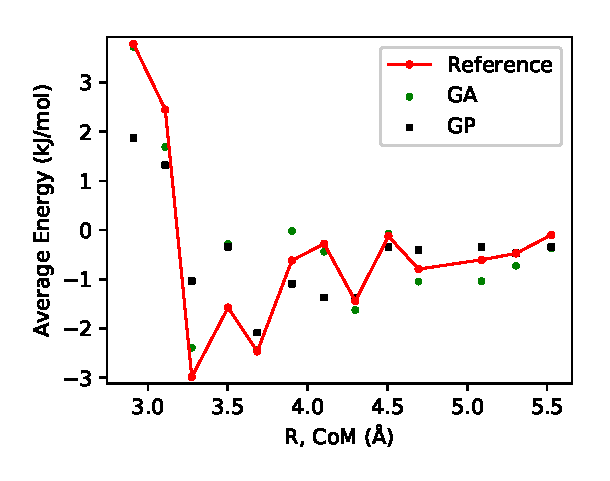
\includegraphics[width=0.45\textwidth]{media/B1_Single_Energy_5_predictors.eps}
\caption{\red{A* tree}\old}\label{Fig:A_star_tree}
\end{figure}

In example shown on Fig. \ref{Fig:A_star_tree} the root is the node that contain chromosome received from either GA or ENet. A* tries to produce children nodes according to its selection criterion (details later) and put them in the sorted queue using binary search. Each new node that goes inside the queue finds its place according to fitness function - lowest first, therefore queue is always sorted. Extraction from queue works exactly as for stack: using pop(). At each iteration A* pops the best child from queue and tries to create its children according to selection criterion and according to correlation coefficients list. Each successfully created child node goes into queue. Algorithm remembers the best node and stops when queue is empty or its working time without improving best node exceeds some value assigned as its parameter.\\
\textit{A* selection criteria.} There are few predefined stopping criteria for algorithm:
Fast: each newly created node compares with best node and goes into queue only if it has better fitness. Algorithm works as one branch of depth first search in this case.
Parent: if newly created node is better than its parent it goes to queue.
Level: if the fitness of newly created node is the best that exist on its level (see \ref{Fig:A_star_tree}) it goes into queue. At the same time when node pop() from queue its fitness compares with best for its level since by the time algorithm reached that node level's fitness could be improved already and this node does not agree with selection criteria. This approach gives good balance between computation speed and accuracy of the fit and has been used for most our computations.
Slow: all nodes produced go to queue and algorithm becomes breadth first search. It scans through all tree and can find the best solution. However, its time complexity O(n**k) where k - deepest level and n - number of variables makes it unmanageable in most cases. \\

\textit{Backward elimination}\old \\

\textit{After GA} \old we have desired and relatively small number of features. I we want to use elastic net instead we can vary its regularization strength and obtain desired number of features but not exact. Then this number of variables can be decreased to required 






\begin{table}[h]
\centering
\caption{Correlation matrix example for 5 variables}\label{Correlation_matrix}
\begin{tabular}{|l|l|l|l|l|l|}
\hline
� & X1 & X2 & X3 & X4 & X5 \\
\hline
X1 & 1.00 & 0.95 & 0.90 & 0.30 & 0.20 \\
\hline
X2 & 0.95 & 1.00 & 0.85 & 0.70 & 0.30 \\
\hline
X3 & 0.90 & 0.85 & 1.00 & 0.60 & 0.40 \\
\hline
X4 & 0.30 & 0.70 & 0.60 & 1.00 & 0.25 \\
\hline
X5 & 0.20 & 0.30 & 0.40 & 0.25 & 1.00 \\
\hline
\end{tabular}
\end{table}




\section{Results and discussion}

The last part summarizes results in report file which include n models 
with corresponding fitting coefficients and creates plots that represent 
prediction of each model using only test set. It also compares our fit 
with gaussian process fit accomplished using the same training set. In 
order to have manageable number of features we have to restrict max power to some reasonable number. Our experiments show that for single distance max power M$_{1}$ from (\ref{eq:tip3p}) value 15 will be sufficient. For features that contain product of distances max power M$_{2}$ from (\ref{eq:tip3p}) 
equal to 7. Increasing those number to greater value does not give any 
significant improvement, but augments number of features and slows down 
the fitting procedure. Table~\ref{Tab:systems}.

\begin{table*}
\caption{Systems and models}\label{Tab:systems}
\begin{tabular*}{\textwidth}{l @{\extracolsep{\fill}} ccccc}
%\begin{tabular}{l*{6}{c}r}
\hline
System & A & B1 & B2 & C & D\\
\hline
Github nickname & set2.x & set6.x & set6.x & set4.x & \\
\hline
$G$ & 1 & 1 & 2 & 2 & \\
\hline
$M_1$ & 15 & 15 & 15 & 15 & \\
\hline
$M_2$ & 0 & 0 & 7 & 7 & \\
\hline
Chemical composition & (H$_2$O)$_2$ & (H$_2$O)$_2$ & (H$_2$O)$_2$ & (H$_2$O)$_3$ & \\
\hline
No. of unique features & & & & &\\
\hline
Ref. energy & TIP3P & MP2 & MP2  & BLYP+D/mo-TZV2P & \\
\hline
Configurations & Grid & $R_{OO}$ bins & $R_{OO}$ bins & AIMD\\
\hline
\end{tabular*}
\end{table*}

Refer to SI for a discussion of LASSO - a special case of EN.


\subsection{System A: TIP3P water dimer}

We would like to show that our algorithm recovers the correct analytic equation from sparse data. In order to test it and to see how well it would find a simple expression, first of all, we used equation~(\ref{eq:tip3p}) to generate data in the interval where the distance between centers of masses of two water molecules varies from 2 to 8 angstrom. We used range of powers from -1 to -15 for features with single distances and the same range for features that contain product of distances. Since all intramolecular distances are just constants they were removed from the set. Also, for simulation we took only a random numbers of coordinates that equally represent each small bin in chosen interval. The bin size was 0.2 angstrom. Initial number of features was 135 + 1008 = 1143. After performing dimensionality reduction genetic algorithm started with 45 + 245 = 290 features and 69 training points per bin with total number of training records equal to  2139. Initial chromosome size was 20 and number of individuals in population was equal to 100. At the and of code execution the exact linear fit with 5 variables and original coefficients were recovered.

Please see Eq.~(\ref{eq:tip3p})

\begin{eqnarray} \label{eq:tip3p}
&E(R_i) = \frac{c_0}{R_{O_1O_2}^{12}}-\frac{c_1}{R_{O_1O_2}^6} + \frac{c_2}{R_{O_1O_2}} - \nonumber
\\
& - c_3(\frac{1}{R_{O_1H_{21}}}+\frac{1}{R_{O_1H_{22}}}+\frac{1}{R_{O_2H_{11}}}+\frac{1}{R_{O_2H_{12}}}) + \nonumber
\\
& + c_4(\frac{1}{R_{H_{11}H_{21}}}+\frac{1}{R_{H_{11}H_{22}}}+\frac{1}{R_{H_{12}H_{21}}}+\frac{1}{R_{H_{12}H_{22}}})
\end{eqnarray}

\subsection{System B: water dimer}

In this part, we focus on two water molecules model. First of all, we need to analyze how RMSE of the function obtained from fitting procedure depends on number of predictors. In simplest case (System B1 Table \ref{Tab:systems}) we have only the first term of equation (\ref{eq:tip3p}). Fig. \ref{Fig:B1_RMSE} shows that if we have a fit with more than 6 variables, RMSE decreases very slightly. If we were to examine what machine learned from dataset first of all it would be wise to compare classic model given by equation (\ref{eq:tip3p}) with newly found fit. For 5 predictors, the results are summarized in Table \ref{Tab:B1 coefficients}. Its RMSE=0.0007068 Ha is even better than the one obtained with classic formula which is 0.0007428 Ha. Since algorithm saves all explored states, we discovered that there are many states with similar goodness of the fit. The one described above is just the best result obtained for this particular configuration (training points are in the interval 2.8A to 5.6A).

\begin{figure}
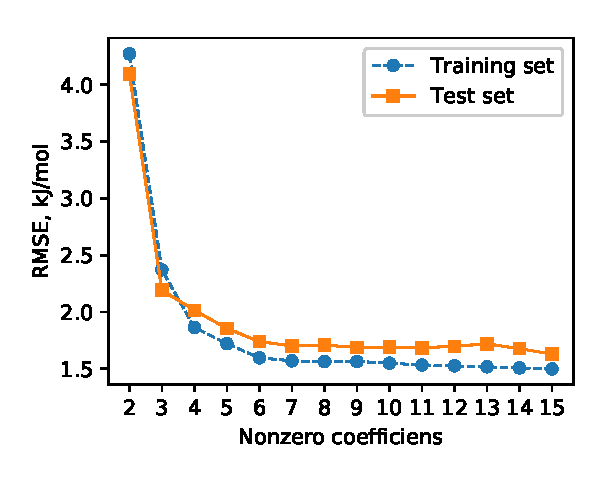
\includegraphics[width=0.45\textwidth]{media/B1_Single_GA_PATH_RMSE.eps}
\caption{Dependence of RMSE on the number of predictors. GA + A* search. System B1}\label{Fig:B1_RMSE}
\end{figure}

\begin{figure}
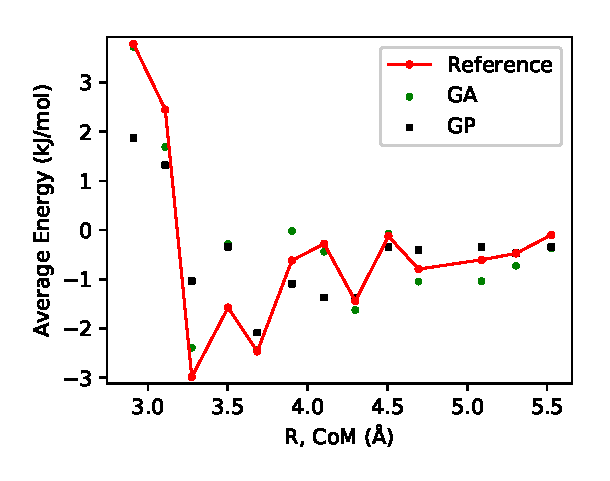
\includegraphics[width=0.45\textwidth]{media/B1_Single_Energy_5_predictors.eps}
\caption{Dependence of enegry on the average disdance between centers of masses. Fit for 5 predictors obtained by GA + A* search and gaussian process. System B1}\label{Fig:B1_Energy}
\end{figure}

\begin{figure}
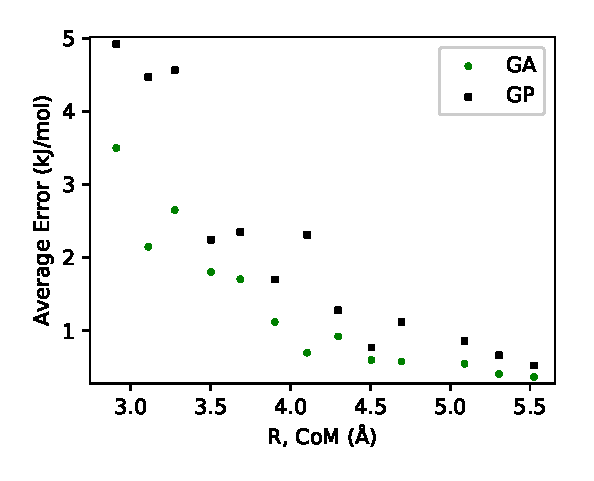
\includegraphics[width=0.45\textwidth]{media/B1_Single_Error_5_predictors.eps}
\caption{Dependence of error on the average disdance between centers of masses. Fit for 5 predictors obtained by GA + A* search and gaussian process. System B1}\label{Fig:B1_RMSE_5_predictors}
\end{figure}

\begin{figure}
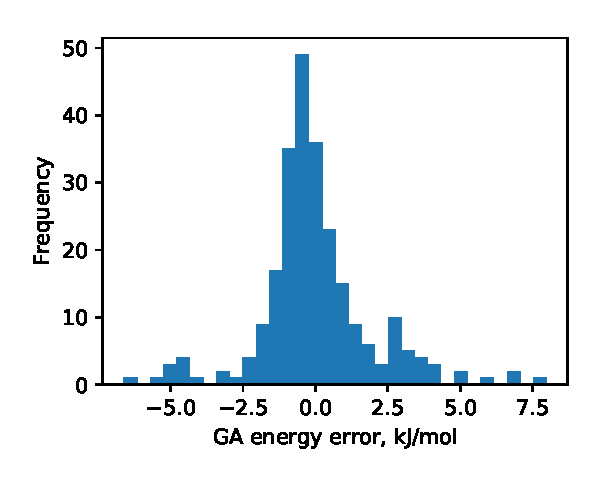
\includegraphics[width=0.45\textwidth]{media/B1_GA_energy_error_histogram_5_predictors.eps}
\caption{Energy error histogram. Fit for 5 predictors obtained by GA + A* search. System B1}\label{Fig:B1_histogram_5_predictors}
\end{figure}

\begin{table}
\caption{Final five-feature fit for system B1 obtained with GA and A* search.}\label{Tab:B1 coefficients}
\begin{tabular*}{0.45\textwidth}{c @{\extracolsep{\fill}} ccc}
%{ccc}
%\begin{tabular}{l*{6}{c}r}
\hline
Distance & Power, $n$ & Coefficient, $Ha\cdot\AA^n$ \\
\hline
O-O & 15 & 10277.7 \\
\hline
O-H & 1 & -0.1348 \\
\hline
O-O & 1 & 0.2726 \\
\hline
H-H & 1 & 0.06622 \\
\hline
H-H & 7 & 0.04201 \\
\hline
\end{tabular*}
\end{table}

In order to analyze deeper system B, we extended our previous model to two terms (System B2 Table  \ref{Tab:systems}) of equation~(\ref{eq:tip3p}). Second term might be useful if there exists dependence between our features generated using first part of equation~(\ref{eq:tip3p}). In this case, the second term will improve the goodness of the fit.

% B2
\begin{figure}
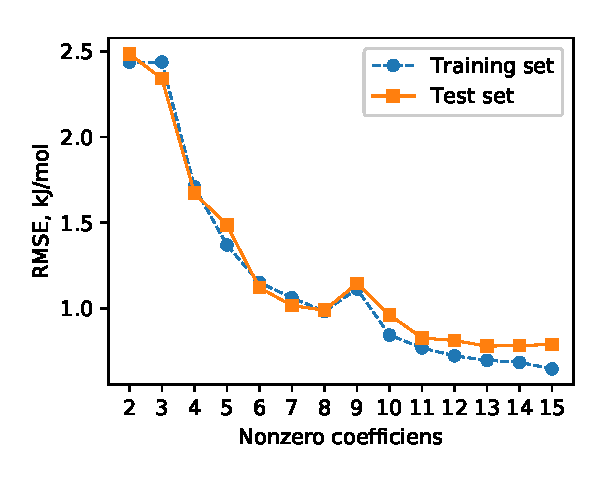
\includegraphics[width=0.45\textwidth]{media/B2_GA_PATH_RMSE.eps}
\caption{Dependence of RMSE on the number of predictors. GA + A* search. System B2}\label{Fig:B2_RMSE}
\end{figure}

\begin{figure}
\includegraphics[width=0.45\textwidth]{media/B2_Energy_12_predictors.eps}
\caption{Dependence of enegry on the average disdance between centers of masses. Fit for 8 predictors obtained by GA + A* search and gaussian process. System B2}\label{Fig:B2_Energy_12_predictors}
\end{figure}

\begin{figure}
\includegraphics[width=0.45\textwidth]{media/B2_Error_12_predictors.eps}
\caption{Dependence of error on the average disdance between centers of masses. Fit for 8 predictors obtained by GA + A* search and gaussian process. System B2}\label{Fig:B2_RMSE_12_predictors}
\end{figure}

\begin{figure}
\includegraphics[width=0.45\textwidth]{media/B2_GA_energy_error_histogram_12_predictors.eps}
\caption{Energy error histogram for 8 predictors. Fit obtained by GA + A* search. System B2}\label{Fig:B2_histogram_12_predictors}
\end{figure}

% B2 VIP 
\begin{figure}
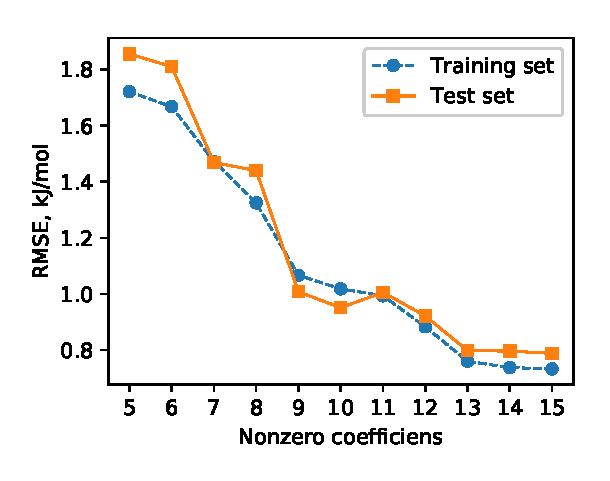
\includegraphics[width=0.45\textwidth]{media/B2_VIP_GA_PATH_RMSE.eps}
\caption{Dependence of RMSE on the number of predictors. GA + A* search. System B2 with fixed 5 best predictors from system B2}\label{Fig:B2_VIP_RMSE}
\end{figure}


For the same number of predictors, lets say 5 system B2 gives better goodness of the fit than system B1 (RMSE.B1 = 0.0007068 Ha and RMSE.B2 = 0.0005661)   
The algorithm chose 3 out of 5 features that contain product of distances which signifies that they are not completely independent and there exists some relationship between them. Plot of RMSE vs. number of nonzero coefficients for system B2 \ref{Fig:B2_RMSE} shows that line becomes gentle approximately near 12. Increasing number of predictors after 12 does not improve significantly fitting results. Coefficients for that particular fit are shown in Table \ref{Tab:B2 coefficients} as well as links to figures that describes features that contain products of distances (Fig. \ref{Fig:B2 Dist}). Plot of average error vs. distance between centers of masses, average energy vs. distance between centers of masses for system B2 and gaussian process are Fig. \ref{Fig:B2_RMSE_12_predictors} and \ref{Fig:B2_Energy_12_predictors} respectively and energy error histogram is represented by Fig. \ref{Fig:B2_histogram_12_predictors}


\begin{table}[h]
\caption{Coefficients for two terms of equation (\ref{eq:tip3p}) with distances description}
\label{Tab:B2 coefficients}
\begin{tabular}{|l|l|l|l|l|l|}
\hline
\textbf{Dist 1} & \textbf{Power 1} & \textbf{Dist 2} & \textbf{
Power 2} & \textbf{Coef $Ha\cdot\AA^n$} & \textbf{Figure} \\
\hline
H-H & -1 & - & - & 0.1517 & - \\
\hline
O-H & -1 & - & - & -0.1617 & - \\
\hline
O-O & -1 & O-H & -1 & 0.9413 & Fig. \ref{Fig:B2 Dist} a) \\
\hline
O-H & -1 & H-H & -1 & -0.4133 & Fig. \ref{Fig:B2 Dist} b) \\
\hline
H-H & -3 & - & - & 0.9059 & - \\
\hline
O-O & -3 & - & - & -5.6737 & - \\
\hline
H-H & -3 & - & - & -0.8635 & - \\
\hline
O-O & -3 & - & - & 6.2834 & - \\
\hline
O-H & -4 & H-H & -4 & 1.0343 & Fig. \ref{Fig:B2 Dist} b) \\
\hline
O-O & -15 & - & - & -1800 & - \\
\hline
H-H & -7 & - & - & 0.09381 & - \\
\hline
O-O & -1 & - & - & 0.007361 & - \\
\hline
\end{tabular}
\end{table}

\begin{figure}
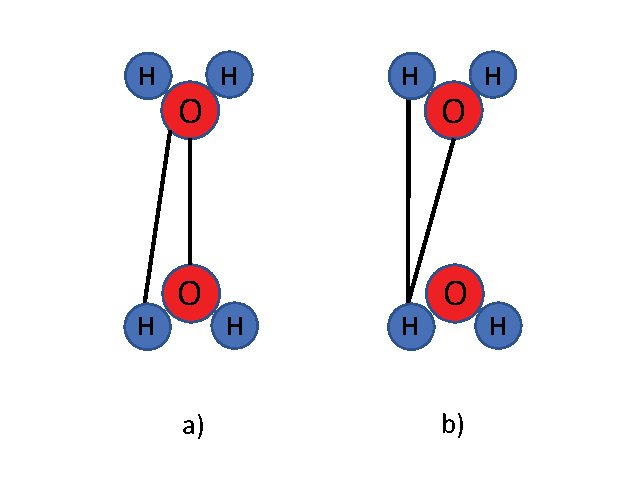
\includegraphics[width=0.45\textwidth]{media/water_distances_1.eps}
\caption{Features description. Model B2. Fig. a) shows the feature that contains the product of O-O and O-H imtermolecular distances. Fig. b) shows the feature that contains the product of O-H and H-H distances.}\label{Fig:B2 Dist}
\end{figure}

\begin{figure}
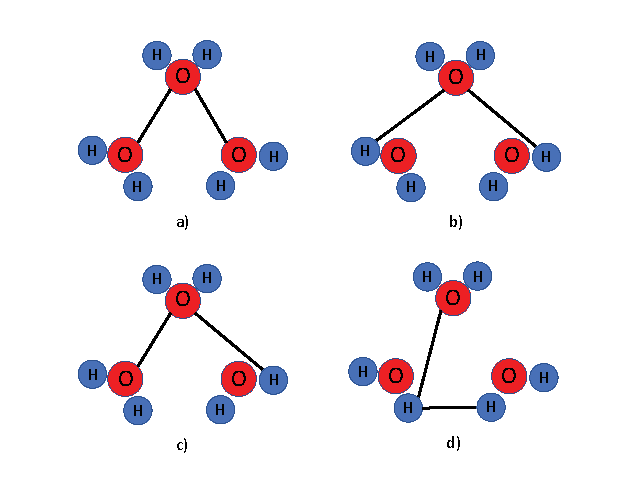
\includegraphics[width=0.45\textwidth]{media/water_distances_2.eps}
\caption{Features description. Model C. Fig. Four a), b), c) and d) represent four different features that contain products of distances O-O * O-O, O-H * O-H, O-O * O-H  and O-H * H-H respectively.}\label{Fig:C Dist1}
\end{figure}

\subsection{System C: three water molecules}

After four predictors increasing numbers of features does not give significant improvement in fitness. What is remarkable that best fit chosen by algorithm contains the same powers for each distance within one complex feature that contains product of distances. Hopefully it is not coincidence because for different results with number of predictors in range from two to ten all "double" features contain products of distances with the same powers. Coefficients and feature descriptions are in Table \ref{Tab:C coefficients}

\begin{figure}
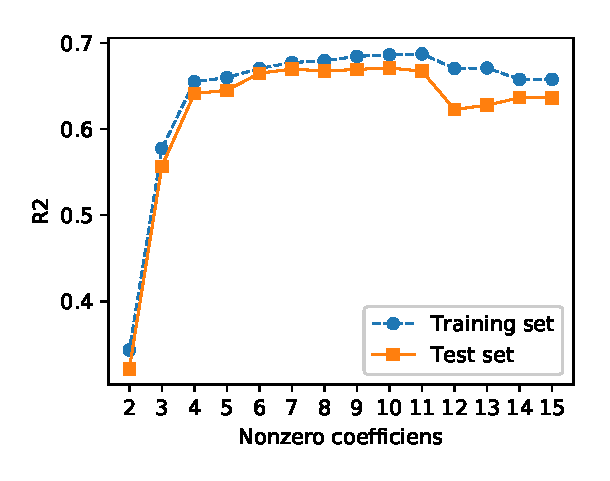
\includegraphics[width=0.45\textwidth]{media/C_GA_PATH_R2.eps}
\caption{Dependence of R2 on the number of predictors. GA + A* search. System C}\label{Fig:C_R2}
\end{figure}

\begin{figure}
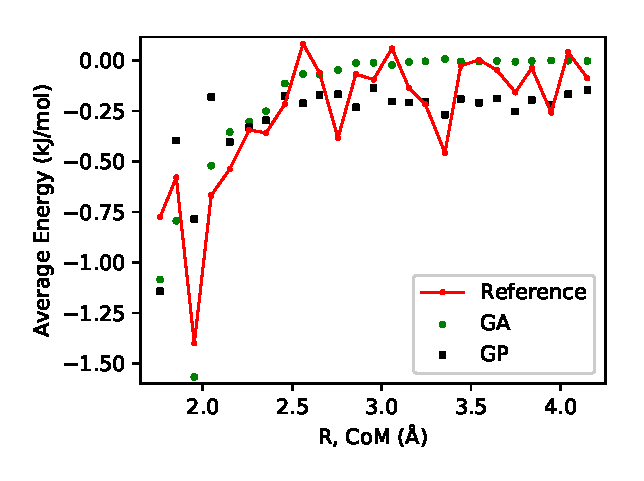
\includegraphics[width=0.45\textwidth]{media/C_Energy_4_predictors.eps}
\caption{Dependence of enegry on the average disdance between centers of masses of molecules to center of mass of the system. Fit for 4 predictors obtained by GA + A* search and gaussian process. System C}\label{Fig:C_Energy_4_predictors}
\end{figure}

\begin{figure}
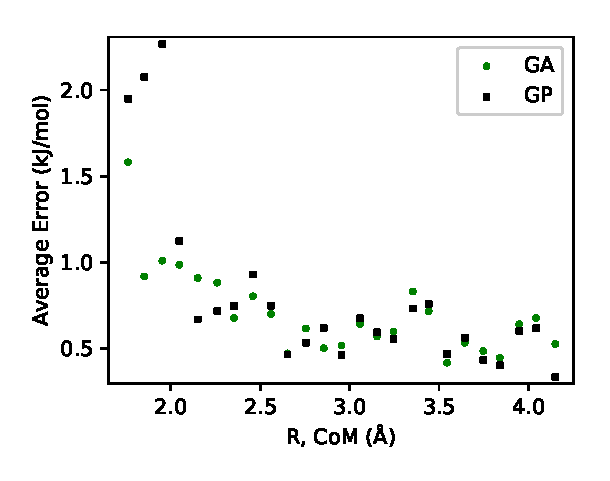
\includegraphics[width=0.45\textwidth]{media/C_Error_4_predictors.eps}
\caption{Dependence of error on the average disdance between centers of masses of molecules to center of mass of the system. Fit for 4 predictors obtained by GA + A* search and gaussian process. System C}\label{Fig:C_RMSE_4_predictors}
\end{figure}

\begin{figure}
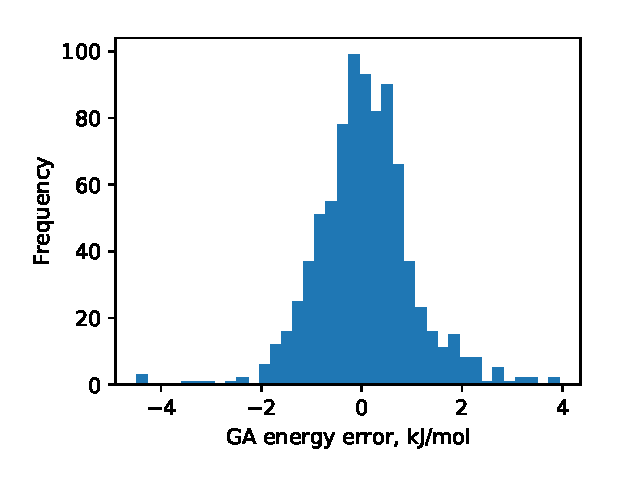
\includegraphics[width=0.45\textwidth]{media/C_GA_energy_error_histogram_4_predictors.eps}
\caption{Energy error histogram. Fit for 4 predictors obtained by GA + A* search. System C}\label{Fig:C_histogram_4_predictors}
\end{figure}

\begin{table}[h]
\caption{Coefficients for system C according to two first terms of equation (\ref{eq:tip3p}) with distances description and corresponding number of distances and powers}
\label{Tab:C coefficients}
\begin{tabular}{|l|l|l|l|l|l|}
\hline
\textbf{Dist 1} & \textbf{Power 1} & \textbf{Dist 2} & \textbf{
Power 2} & \textbf{Coef $Ha\cdot\AA^n$} & \textbf{Figure} \\
\hline
O-H & -3 & O-H & -3 & 0.3495 & Fig. \ref{Fig:C Dist1} b) \\
\hline
O-O & -3 & O-O & -3 & 1.5937 & Fig. \ref{Fig:C Dist1} a) \\
\hline
O-O & -3 & O-H & -3 & -0.9107 & Fig. \ref{Fig:C Dist1} c) \\
\hline
O-H & -4 & H-H & -4 & -0.2013 & Fig. \ref{Fig:C Dist1} d) \\
\hline
\end{tabular}
\end{table}


\subsection{Comparison with Gaussian process}

Another interesting aspect is to compare our results with Gaussian 
process. At the same time, we have to investigate one of our goals: can 
our algorithm predict in regions where there are no training points, in 
other words can we use it to interpolate and extrapolate. To do this we 
removed training points from some regions. In the following example 
simulation will be performed in the region where average distance 
between center of masses of two water molecules spans $[$2.4 .. 15$]$ 
angstrom. However, we removed all data in region $[$5 .. 7$]$ angstrom 
to see how interpolation works and at the edge region $[$9 .. 15$]$ 
angstrom to observe extrapolation. It has to mentioned that we kept test 
points in entire region $[$2.4 .. 15$]$ angstrom. In addition, predicted 
values of energy obtained by Gaussian process are to be compared with 
our method. 

\begin{figure}[h]
\centering
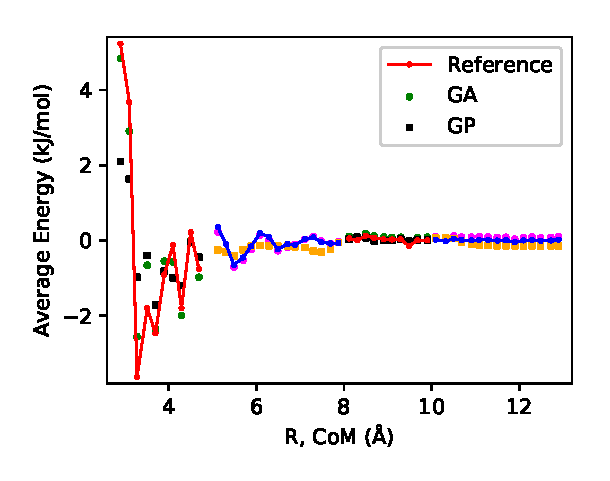
\includegraphics[width=0.45\textwidth]{media/B1_gap_Energy_6_predictors.eps}
\caption{\textit{Dependence of energy on the average disdance between centers of masses. Fit for 6 predictors obtained by GA + A* search and Gaussian process. System B1. Trained region $[$2.4..5$]$, 
$[$7..9$]$ angstrom, test region $[$2.4..15$]$ angstrom}}
\label{Fig:B1_gap_energy_6_predictors}
\end{figure}

\begin{figure}[h]
\centering
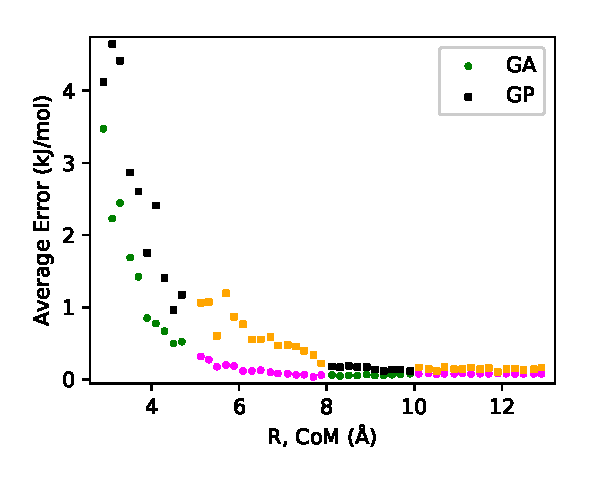
\includegraphics[width=0.45\textwidth]{media/B1_gap_Error_6_predictors.eps}
\caption{\textit{Dependence of error on the average disdance between centers of masses. Fit for 6 predictors obtained by GA + A* search and Gaussian process. System B1. Trained region $[$2.4..5$]$, 
$[$7..9$]$ angstrom, test region $[$2.4..15$]$ angstrom}}\label{Fig:B1_gap_RMSE_6_predictors}
\end{figure}

\begin{figure}[h]
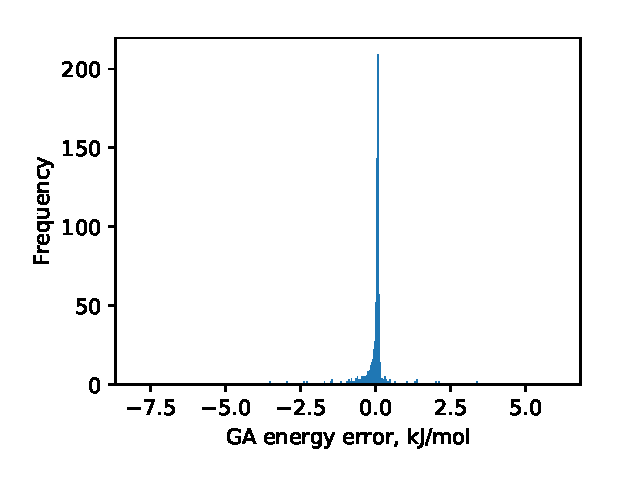
\includegraphics[width=0.45\textwidth]{media/B1_gap_GA_energy_error_histogram_6_predictors.eps}
\caption{\textit{Energy error histogram. Fit for 6 predictors obtained by GA + A* search. System B1. Trained region $[$2.4..5$]$, 
$[$7..9$]$ angstrom, test region $[$2.4..15$]$ angstrom}}\label{Fig:B1_gap_histogram_6_predictors}
\end{figure}


Fig. 8 and 9 clearly show that in trained region $[$5..7$]$ both 
algorithms give pretty well prediction where error is relatively small 
and predicted energy almost identical with true energy. In the 
$[$2.4..5$]$ angstrom region error is greater as well as deviation of 
predicted energy since on short distances the behavior of two water 
molecules system is much more complex and true energy function has more 
complex shape. However, if we examine two regions where there are no 
training points we can see a big difference in prediction. Our linear 
model is still good: predicted energy values are close to true energy 
and level of the error is almost the same as in adjacent trained region. 
Gaussian process behaves differently: error goes up and values of 
predicted energy also higher, especially et the edge region $[$9..15$]$ 
angstrom. It can be observed from histogram on Fig. 10 that error 
distribution is reasonable since the most frequently occurred error 
values are close to zero.


Similarly, to those results Fig. 11, 12, 13 represent the model 
according to (4) with 6 predictors and the same other parameters. The 
fit is even better than if we used eq. (3), but general behavior is 
similar.




Another important aspect is to examine the dependence of goodness of fit 
on number of training points. To do that we used model based on eq. (4) 
and trained regions $[$2.4..5$]$, $[$7..9$]$ and test region $[$2.4 .. 
15$]$ angstrom. However, instead of using all training points we used 10 
different fits with number of training points from 10\% of initial 
number up to 100\% with the step 10\%. Both linear model and Gaussian 
process were examined in equal conditions. The results are represented 
by Fig. 14 and 15. It can be clearly seen that Gaussian process requires 
more training points to obtain reasonable prediction. Linear model 
behaves better when we used reduced number of training points and gave 
reasonable results even at 10\% of initial set. All points were chosen 
randomly for each small interval that represent some value measured as 
average distance between the centers of masses of two water molecules. 

\begin{figure}[h]
\centering
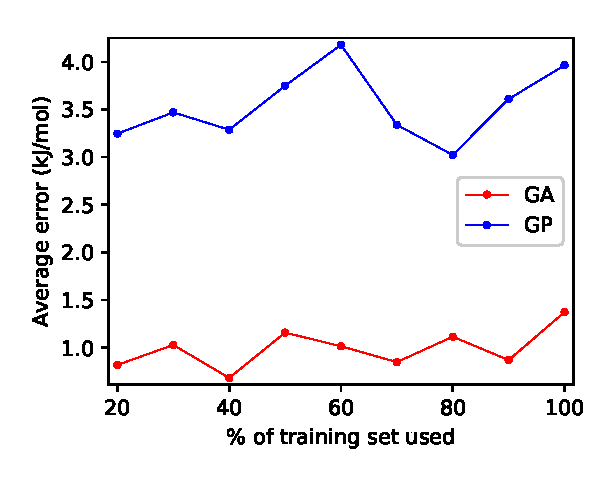
\includegraphics[width=0.45\textwidth]{media/B2_12_predictors_RMSE_vs_percentage_of_training_set_used.eps}
\caption{RMSE vs. \% of usage of training points. System B2 with 12 predictors and Gaussian process. Trained and test regions [2.8..5.6] angstrom}
\label{Fig:B2_fractions}
\end{figure}

\section{Conclusions}

In this work, we proposed a new machine learning strategy to reproduce the interaction energy between molecules based on a limited training set of accurate quantum mechanical data. Unlike existing machine learning techniques, the new methodology is designed to incorporate physically relevant information into the model while still retaining its high flexibility. In addition to this, the learning strategy is developed around a strict control of overfitting and thus selects only the most important components of model. 
%This goal is achieved through a combination of modern artificial intelligence algorithms including genetic and elastic net algorithms.
It is demonstrated, using water molecules as an example, that this approach recovers fundamental physical laws that govern intermolecular interactions. As a result, the obtained models do not only reproduce quantum mechanical energies in the region spanned by the training set configurations but are also capable of extrapolating well outside this region -- a remarkable achievement for machine learning in molecular modeling. Moreover, it is shown that incorporating physically motivated features into the model drastically reduces the number of reference data points in the training set without sacrificing the quality of predictions. 
%improves predictive power of machine learning for molecular/materials modeling. 
In the future, the approach presented here will be extended to systems of strongly interacting atoms 
%in gas-phase molecules, condensed phase systems, and materials
that may require incorporating more complex nonlinear physical features. 
% reformulation of the procedure in the Bayesian framework analogous to that of GPR (kernel)


\section{Computational methods}

\textbf{Gaussian process regression. }To better understand the 
accuracy and the performance of our method it would be nice to compare 
its results with the ones obtained by using another machine learning 
algorithms such as artificial neural network or gaussian process. For 
this article, Gaussian process has been chosen since it can "\,mimic" 
the shape of almost any complex function. We used 
GaussianProcessRegressor from sklearn.gaussian\_process which is the 
implementation of Gaussian Processes for Machine Learning by Rasmussen 
and Williams. During fitting the hyperparameters of the kernel are 
optimized by maximizing the log-marginal-likelihood based on the passed 
optimizer. We used two kernels RBF which is basically Radial-basis 
function or squared-exponential kernel and White Kernel the main use of 
which is to add noise level component to the signal. Those two kernels 
have two crucial parameters: length scale and noise level respectively. 
Varying those parameters, it is possible to find the local maxima of the 
function to achieve the best possible fit. Either optimizer provided by 
scipy.optimize.fmin\_l\_bfgs\_b or user defined optimizer that must have 
specific signature can be used to attune kernels and therefore GP 
regressor to give optimal results. Since local maxima is a function of two main variables, to find optimal solution we used a stochastic hill climbing algorithm with random restart (Fig \ref{Fig:B1_Gaussian_path}). 

\begin{figure}
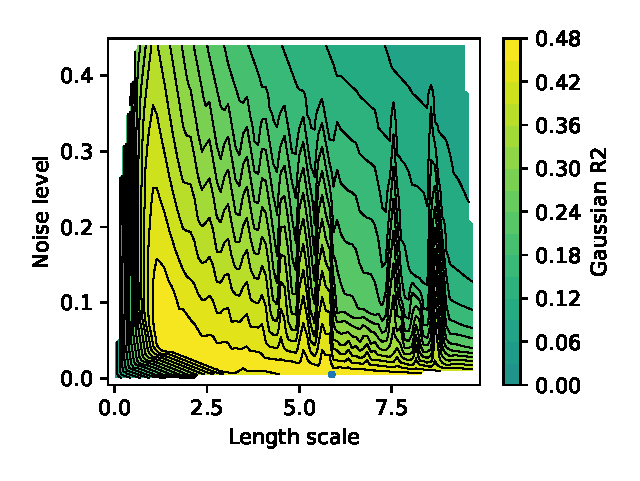
\includegraphics[width=0.45\textwidth]{media/B1_Gaussian_path.eps}
\caption{Gaussian path by stochastic hill climbig with 10 random restarts. Best gaussian result coresponds to blue dot on the graph. System B1}\label{Fig:B1_Gaussian_path}
\end{figure}

\section{Acknowledgments} 

The research was funded by the Natural Sciences and Engineering Research Council of Canada (NSERC) through Discovery
Grants (RGPIN-2016-0505). The authors are grateful to Compute Canada and, in particular, the McGill HPC Centre for computer time.

\bibliography{learn-physics}

%RZK0: uncomment the switch to separate SI from the main text
%\else % maintext - SI switch

\newpage
\clearpage
%\widetext
\setcounter{figure}{0}
\setcounter{page}{1}
\renewcommand{\thefigure}{S\arabic{figure}}


\section{LASSO} 

We have explored performance of least absolute 
shrinkage and selection operator (LASSO) method for the feature 
selection stage of the training algorithm. LASSO is a special case of 
the elastic net regularization with ZZZ coefficient being set to zero. 
We found that LASSO, based on both forward stepwise and least angle 
regression, tends to drop important features that are somewhat collinear 
to those already selected. As a result, the final list selected by LASSO 
contains too few features.

In a multiple regression model multicollinearity indicates that the 
collinear independent variables are somehow related. The presence of 
multicollinearity within the set of features causes many problems in the 
understanding the significance of individual independent features in our 
regression model. Our feature set is generated in such a way that it is 
impossible to avoid collinearity and multicollinearity since basically 
we have set of distances raised to different powers. The variance 
inflation factors (VIF) can prof that we have multicollinearity issues 
in our set. It allows a quick estimation of how much a variable is 
contributing to the standard error in our regression model. VIF is very 
large when significant multicollinearity issues exist. Multicollinearity 
can lead to less reliable probability values and larger confidence 
intervals.


\red{Best first search tree algorithm with different parameters for convergence;
Stochastic hill climbing algorithm with random restart;
Genetic algorithm: two types of selection for crossover, using Pearson  correlation coefficients for mutation;

}
\textbf{Best fit algorithm.} Schematically the algorithm looks like 
following pseudocode:

\textit{while found:}

\textit{found = False}

\textit{for feature in features:}

\ \ \ \ \textit{for alternate in feature.alternates:}

\ \ \ \ \ \ \ \ \textit{Replace\_temporarely(alternate, features)}

\ \ \ \ \ \ \ \ \textit{new\_score = Score(features)}

\ \ \ \ \ \ \ \ \textit{if new\_score $<$ best\_score:}

\ \ \ \ \ \ \ \ \ \ \ \ \textit{found = True}

\ \ \ \ \ \ \ \ \ \ \ \ \textit{Replace\_permanently(alternate, 
features)}

\ \ \ \ \ \ \ \ \ \ \ \ \textit{best\_score = new\_score}

\ \ \ \ \ \ \ \ \ \ \ \ \textit{continue}

where: 

feature.alternates - a list of alternating (most correlated) features 
created previously in correlation analysis part

Replace\_temporarely - temporarily replacement of current feature by its 
alternative from the list

Replace\_permanently - permanent replacement of current feature by its 
alternative. It also means that the list feature.alternates is been 
replaced too by appropriate one from correlation analysis

Score - some fitness function that evaluates the goodness of the fit. 
For linear model we used OLS and for exponential fit we used 
scipy.optimize.least\_squares.


\fi % maintext - SI switch

\end{document}
